% ************ Chapter 3 ************
\chapter{Requisitos} 
\label{cap:3}
Neste capítulo é apresentado todos os levantamentos de requisitos feitos, o estudo do sistema anterior e a lista de requisitos final.

\section{Primeiro levantamento de requisitos}
Antes de iniciar qualquer tipo de desenvolvimento ou implementação, era fulcral também definir uma lista de requisitos, que descrevesse de uma forma muito exata e clara o que se esperava que a solução implementada fosse. Logo na primeira reunião foi entregue um primeira lista de requisitos dividida em dois tipos diferentes: os primeiros são designados por Requisitos Absoluto que são requisitos com um grande nível de detalhe sobre as suas características e perspetivas. Os segundos designamos por Requisitos Indexados, sobre os quais não se tem certeza sobre a totalidade das suas características ou dependem da informações externas. Os requisitos pertencentes a este último grupo devem passar por um processo de definição de modo a que se tornem também requisitos absolutos.
No final da primeira reunião a lista de requisitos entregue foi a seguinte\\
\\
Requisitos absolutos:
\begin{itemize}
	\item A aplicação só poderia ser acessível da rede interna;
	\item Uso de uma base de dados relacional;
	\item Registo do horário de entrada e saída dos colaboradores;
	\item Registo do peso e ponto de recolha de onde vinha a matéria prima;
	\item Registo do peso de cera, metal e plástico de uma produção, bem como o colaborador associado;
	\item Registo do peso do produto final acabado;
	\item Registo da saída de produto acabado e cliente a quem foi vendido;
	\item Impressão de uma segunda via dos códigos de barras já impressos referente a uma recolha ou um produto acabado;
	\item Incremento do peso de uma recolha efetuada anteriormente;
	\item Zona protegida por IDentifier (ID\label{sym:ID})e \textit{Password} para a consulta dos registos feitos;
	\item Possibilidade de editar e apagar registos já feitos;
	\item \textit{Script} de analise da coerência dos dados registados.
\end{itemize}
Requisitos indexados:
\begin{itemize}
	\item Deveria ocorrer uma melhoria do \textit{design} da base de dados;
	\item A aplicação deveria ser acessível em dispositivos moveis e computadores;
	\item Desenvolvimento de uma funcionalidade que permitisse o incremento do peso de uma recolha.
\end{itemize}
Terminada esta reunião foi iniciado um processo de estudo do sistema atualmente implementado, o funcionamento da fábrica de forma a desindexar os requisitos indexados e determinar novos requisitos por forma a ter a melhor descrição possível do sistema a ser implementado.

\section{Estudo do sistema existente}
O sistema existente na empresa foi construído com recurso ao Microsoft Access. Era compostos por 5 ecrãs destintos utilizados para recolher a informação gerada na fábrica. Um dos aspetos evidentes desde inicio é a não-coesão visual dos elementos, como demonstrado na figura \ref{fig:app_access}.

\begin{figure}[h!]
	\centering
	
	\begin{subfigure}[c]{0.3\linewidth}
		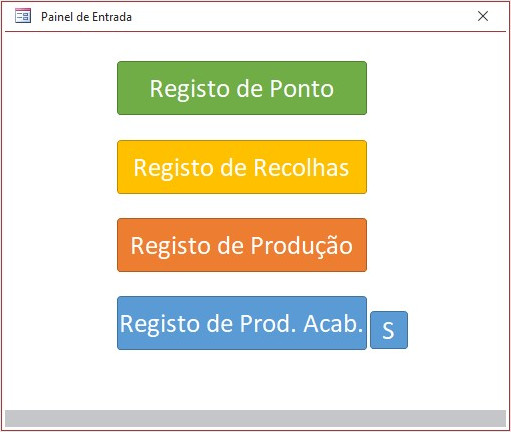
\includegraphics[width=\linewidth]{figuras/AppAccess/0-MenuInicial.jpg}
		\caption{Menu incial}
	\end{subfigure}
	\begin{subfigure}[c]{0.3\linewidth}
		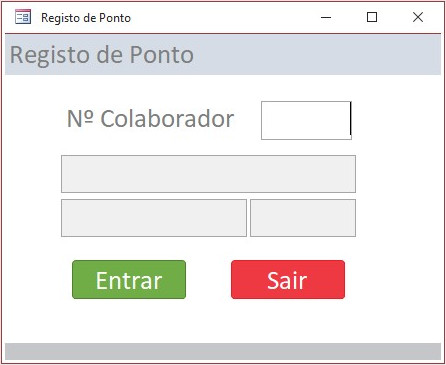
\includegraphics[width=\linewidth]{figuras/AppAccess/1-Ponto.jpg}
		\caption{Ecrã de marcação do ponto}
	\end{subfigure}
	\begin{subfigure}[c]{0.3\linewidth}
		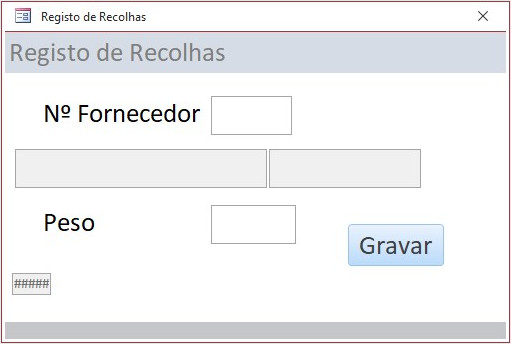
\includegraphics[width=\linewidth]{figuras/AppAccess/2-Recolha.jpg}
		\caption{Ecrã do registo de recolha}
	\end{subfigure}
	\begin{subfigure}[c]{0.3\linewidth}
		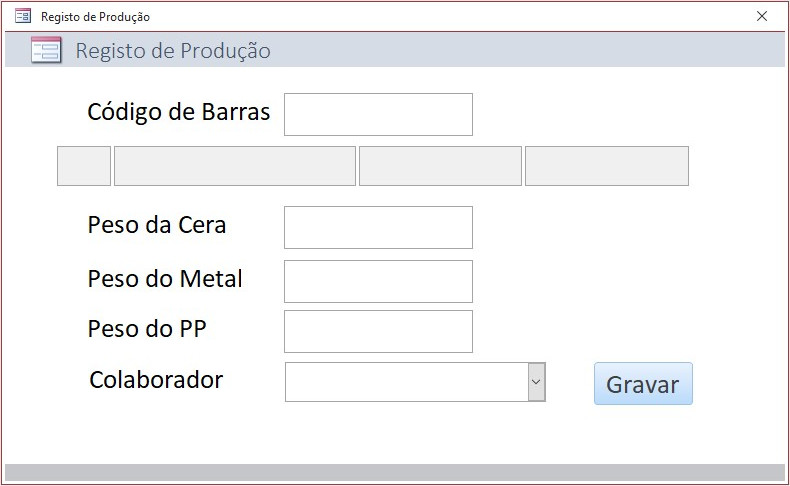
\includegraphics[width=\linewidth]{figuras/AppAccess/3-Producao.jpg}
		\caption{Ecrã do registo de produção}
	\end{subfigure}
	\begin{subfigure}[c]{0.3\linewidth}
		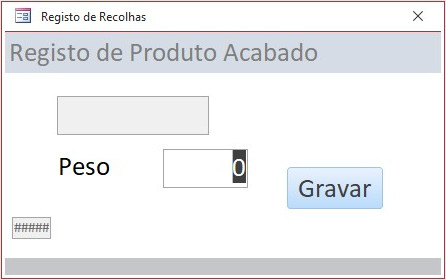
\includegraphics[width=\linewidth]{figuras/AppAccess/4-ProdutoAcabado.jpg}
		\caption{Ecrã do registo de produto acabado}
	\end{subfigure}
	\begin{subfigure}[c]{0.3\linewidth}
		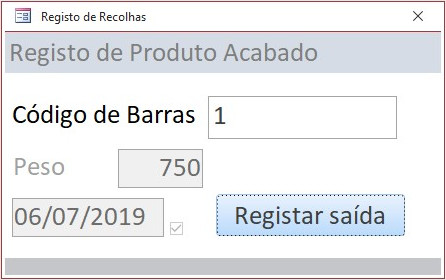
\includegraphics[width=\linewidth]{figuras/AppAccess/5-SaidaProdutoAcabado.jpg}
		\caption{Ecrã do registo de saída de produto acabado}
	\end{subfigure}
	
	\caption{Ecrãs da aplicação existe na empresa.}
	\label{fig:app_access}
\end{figure}

O fluxo dentro deste sistema era bastante simples. Ao executar o ficheiro Microsoft Access, era apresentado diretamente o menu ao utilizador. Este selecionaria a opção referente ao registo que pretendia fazer e uma nova janela surgia com o formulário correspondente. O utilizador preenchia com os dados requeridos e pressionava o botão "Gravar". Em caso de sucesso não era apresentado nenhuma mensagem. Em caso de erro era apresentada uma mensagem com essa informação. Estas mensagens era geradas diretamente pelo sistema de gestão de base de dados e não eram intuitivas. No caso de ser o registo de recolha ou de produto acabado, era ainda apresentado, numa nova janela um código de barras que seria impresso para identificar on elemento registado. Um exemplo do resultado impresso é demonstrado na figura \ref{fig:app_access_cb}.

\begin{figure}[H]
	\centering
	
	\begin{subfigure}[t]{0.4\linewidth}
		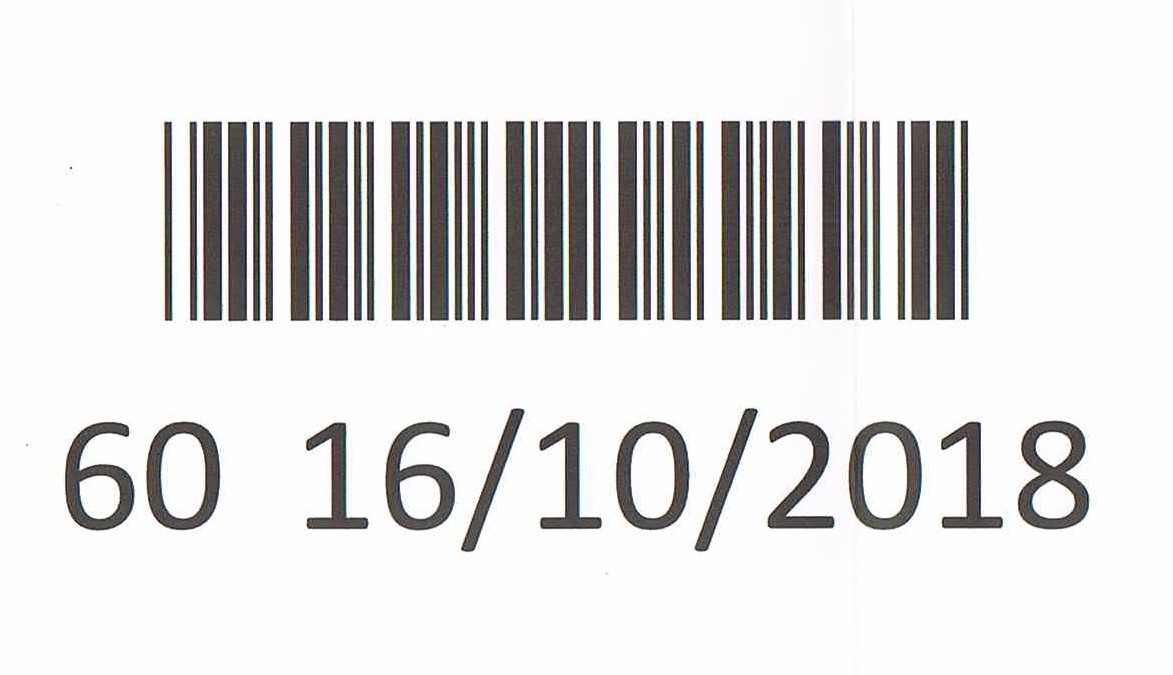
\includegraphics[width=\linewidth]{figuras/AppAccess/2-CodBarras.jpg}
		\label{fig:app_access_cb_recolha}
		\caption{Recolha}
	\end{subfigure}
	\begin{subfigure}[t]{0.4\linewidth}
		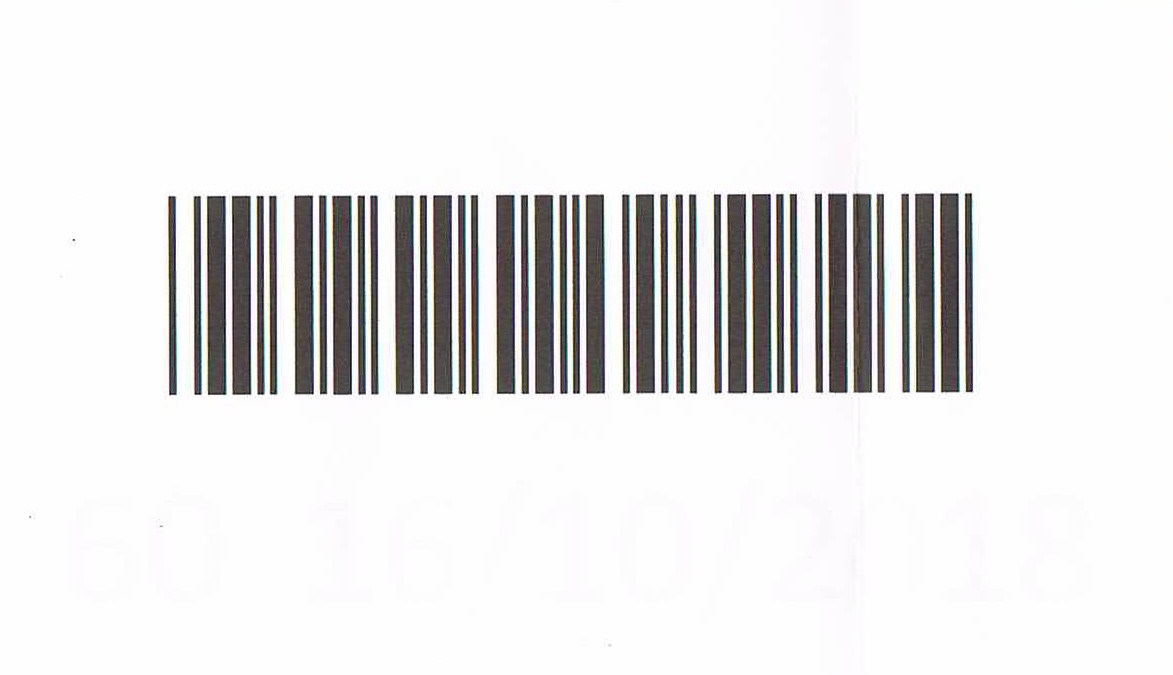
\includegraphics[width=\linewidth]{figuras/AppAccess/5-CodBarras.jpg}
		\label{fig:app_access_cb_prod_acabado}
		\caption{Produto Acabado}
	\end{subfigure}
	
	\caption{Exemplo dos códigos de barras gerados}
	\label{fig:app_access_cb}
\end{figure}
\noindent
Estes códigos de barras deveriam ter estruturas diferentes. O código de barras referente à recolha (figura \ref{fig:app_access_cb} (a) deveria ser constituído pelo código de barras correspondente ao ID da recolha, o ID do ponto de recolha e a data da recolha. Já no caso produto acabado era apenas apresentado o código de barras referente ao ID do mesmo (figura \ref{fig:app_access_cb} (b). A pedido da administração deveria passar a ser apresentado também o ID do produto acabado em formato numérico.\\
Após o estudo da aplicação foi iniciado o estudo da base de dados. Este estudo consistiu em compreender as tabelas que constituem base de dados, as suas relações e a informação que nelas era registada. Foi também solicitado pela empresa sugestões de melhoria do \textit{design} da base de dados com foco na coerência da informação registada.

\section{Modo de implementação do projeto}
Numa das reuniões discutiu-se o modo como o novo sistema deveria ser implementado. No dia em que ocorresse a primeira implementação do novo sistema, este deveria substituir por completo a aplicação construída no Microsoft Access. Isto porque devido à natureza da informação registada e tendo em conta que a base de dados teria a sua estrutura modificada, não era possível existir um período hibrido onde as duas aplicações coexistiram. Assim ficou definido que enquanto o novo sistema não fosse capaz de registar o ponto dos colaboradores, as recolhas efetuadas, as produções feitas, o produtos finalizados e a sua saída, a implementação não iria ocorrer.
Foi definido então que o sistema teria de passar por dois níveis de testes sendo o primeiro os testes de desenvolvimento e o segundo o teste com utilizadores reais de forma a identificar erros não previstos no período de desenvolvimento.

\section{Último levantamento de requisito}
Todos os requisitos da aplicação ficaram definidos no final da primeira semana, à excepção dos requisitos referentes a uma nova funcionalidade que permitisse o incremento do peso de uma recolha. Em algumas recolhas efetuada, o peso total da recolha superava a capacidade de ser pesado de uma só vez, seja pelo peso de matéria prima seja pela quantidade. Apesar de estarmos conscientes desta necessidade foi sugerido deixar a discussão sobre esta nova funcionalidade para o pós primeira implementação. Não se tratava de uma funcionalidade fundamental para o sistema e como tal havia a intenção de estudar a melhor forma de implementar esta solução e que apenas foi discutida na oitava semana do período de estágio. Consistiu na criação de uma nova tabela "Completar Recolha" que iria armazenar o histórico de incrementos feitos numa recolha, para assim poder identificar eventuais erros no registos da informação. Do ponto de vista da aplicação a recolha a ser incrementada seria identificada pelo código de barras impresso anteriormente e deveria ser apresentado ao utilizador o histórico de incrementos referente a essa recolha. Por fim definiu-se que uma recolha registada com o peso de zero quilos deveria redirecionar automaticamente o utilizador para o ecrã do incremento desta recolha após a impressão do primeiro código de barras.

\section{Lista final de requisitos}
Após as todas as reuniões de levantamento de requisitos, chegou-se à seguinte lista composta apenas por requisitos absolutos.
\begin{itemize}
	\item A aplicação só poderia ser acessível da rede interna
	\item A aplicação alojada num servidor físico com Ubuntu Server 18.04
	\item A aplicação WEB desenvolvida em PHP, com o framework Laravel, e em JavaScript;
	\item A aplicação teria de seguir o modelo \textit{Model View Controller} (MVC\label{sym:MVC});
	\item A aplicação deve ser construída de forma modular de forma a facilitar a sua manutenção no futuro;
	\item Uso de uma base de dados relacional, construída com o sistema de gestão de base de dados Microsoft SQL Server e a estrutura aprovada pela administração;
	\item A implementação teria de ser feita em duas fases:
	\begin{itemize}
		\item a primeira onde se substituía totalmente a aplicação existente na fabrica (Registo de ponto, de recolhas, de produção, de produto acabado e de saída de produto acabado);
		\item a segunda fase durante a qual as novas funcionalidades seriam aplicadas incrementalmente;
	\end{itemize}
	\item A aplicação teria de passar por uma fase de testes muito exigente para impedir erros que obrigassem ao uso da base de dados antiga.
	\item Os testes têm de ser divisos em dois níveis:
	\begin{itemize}
		\item Nível 1: testes de desenvolvimento;
		\item Nível 2: testes com utilizadores reais;
	\end{itemize}
	\item O sistema tem de ser graficamente coeso;
	\item O sistema terá de ter um tempo de aprendizagem mínimo no modo de utilização dos funcionários;
	\item O sistema deverá emitir mensagens após cada ação;
	\item As mensagens têm de ter linguagem simples e direta;
	\item O registo do horário de entrada e saída dos colaboradores;
	\item O registo do peso e ponto de recolha de onde vinha a matéria prima;
	\item Impressão de um código de barras com o ID gerado para a recolha inserida, ID do ponto de recolha e data de recolha;
	\item O sistema deve permitir de incrementar o peso de uma recolha;
	\item Se a recolha fosse iniciada com 0 kg é iniciado automaticamente o processo de incremento do peso da recolha que acabou de ser registada;
	\item Após o incremento do peso deveria ser impresso uma segunda via do código de barras dessa mesma recolha;
	\item Registo do peso de cera, metal e plástico de uma produção, bem como o colaborador associado;
	\item Registo do peso do produto final acabado;
	\item Impressão de um código de barras com o ID gerado para a produto final acabado;
	\item Registo da saída de produto acabado e cliente a quem foi vendido;
	\item Impressão de uma segunda via dos códigos de barras já impressos referente a uma recolha ou um produto acabado;
	\item Zona protegida por ID e \textit{Password} para a consulta dos registos feitos;
	\item As tabelas apresentadas na interface da aplicação teriam de ser capazes de refletir alterações na estrutura das tabelas da base de dados;
	\item O sistema deve permitir listar, inserir, editar, apagar e emitir uma segunda via de código de barras de uma \textit{recolha};
	\item O sistema deve permitir listar, inserir, editar e apagar uma \textit{produção};
	\item O sistema deve permitir listar, inserir, editar, apagar e emitir uma segunda via de código de barras de um \textit{produto acabado};
	\item O sistema deve permitir listar, inserir, editar, apagar e desativar um \textit{colaborador};
	\item O sistema deve permitir listar, inserir, editar e apagar um \textit{registo de ponto};
	\item O sistema deve permitir listar, inserir, e apagar um \textit{utilizador};
	\item O sistema deve permitir listar, inserir e editar uma \textit{entidade};
	\item O sistema deve permitir listar, inserir, editar, apagar e desativar um \textit{ponto de recolha};
	\item O sistema deve permitir listar, inserir, editar, apagar e desativar um \textit{cliente};
	\item O sistema deve permitir listar, inserir, editar, apagar e executar uma \textit{analise personalizada};
	\item \textit{Script} de analise da coerência dos dados registados para Pontos de Recolha, Registos de Ponto e Produção.
\end{itemize}